\documentclass[a4paper,12pt,twoside]{article}
\usepackage[T1,T2A]{fontenc}
\usepackage[utf8]{inputenc}

\usepackage{bsumain}
\usepackage{bsudiplomatitle14}
\usepackage{blindtext}

\usepackage{graphicx}
\usepackage{blindtext}
\usepackage{ mathrsfs }
\usepackage[russian,english]{babel}
\usepackage{enumitem}
\usepackage[english,russian]{babel}
\usepackage{amsmath}
\usepackage[top=20mm, bottom=20mm, left=20mm, right=20mm]{geometry}

\author{Деркач Максим Юрьевич}
\title{Оценка надежности криптографических преобразований на основе нейронных сетей}

\begin{document}
	\begin{center}
		{МИНИСТЕРСТВО  ОБРАЗОВАНИЯ  РЕСПУБЛИКИ  БЕЛАРУСЬ\\
			БЕЛОРУССКИЙ ГОСУДАРСТВЕННЫЙ УНИВЕРСИТЕТ\\
			ФАКУЛЬТЕТ ПРИКЛАДНОЙ МАТЕМАТИКИ И ИНФОРМАТИКИ} \\
		{Кафедра математичекого моделирования и анализа данных}
		
	\end{center}
	
	\begin{center}
		\bigskip
		\bigskip
		\bigskip
		\bigskip
		\textbf{Отчёт\\ о прохождении производственной практики\\ для специальности \\
		1-31 81 12«Прикладной компьютерный анализ данных»}
	\end{center}
	
	
	\hfil\hfil\hfil\hfil	магистранта 2года обучения\\
	\bigskip
	\hfil\hfil\hfil\hfil	Деркача Максима Юрьевича\\
	\bigskip
	
	\hfil\hfil\hfil\hfil	Руководитель практики от кафедры\\
	\bigskip
	\hfil\hfil\hfil\hfil	чл.-корр. НАН Беларуси,\\
	\bigskip
	\hfil\hfil\hfil\hfil	доктор физ.-мат. наук, профессор\\
	\bigskip
	\hfil\hfil\hfil\hfil	Харин Юрий Семенович\\
	\bigskip
	
	\hfil\hfil\hfil\hfil	Руководитель практики от организации
	\bigskip
	\hfil\hfil\hfil\hfil	Пьянов Владислав Сергеевич\\
	
	
	
	\begin{center}
		Минск, 2019
	\end{center}
	
	
	\newpage
	
	 {
    \renewcommand{\contentsname}{Оглавление}
    \tableofcontents
  	}
	
	\section{Введение}
	\bigskip
	
	Проблема защиты информации затрагивает практически все сферы деятельности человека. Среди способов защиты информации важнейшим считается криптографический [1]. 
	
	Нейронная криптография - это раздел криптографии, посвященный анализу применения стохастических алгоритмов, особенно алгоритмов искусственных нейронных сетей, для использования в шифровании и криптоанализе.[2] Существуют решения, построенные на основе искусственных нейронных сетей, позволяющие обеспечить доступность данных [3].
	
	Архитектура искусственных нейронных сетей позволяет эффективно проводить работы по распознаванию образов и классификации множества объектов по любым признакам. Кроме того, благодаря хорошо продуманному алгоритму обученные нейронные сети могут достигать чрезвычайно высоких уровней точности. 
	
	Основной целью практики было построить нейронную сеть для апроксимации двоичной (дискретной) функции и провести анализ полученных результатов. 
	
	\newpage
	\section{Перечень задач}
	\bigskip
	
	\begin{enumerate}
		\item Построить генератор двоичных функций на основе полинома Жегалкина.
		\item Построить однослойную нейронную сеть для апроксимации двоичной(дискретной) функции.
		\item Провести компьютерные эксперименты с однослойной нейронной сетью для апроксимации тестовой двойчной функции и криптографического примитива. Провести анализ проведенного эксперимента.
		\item Построить многослойнную нейронную сеть для апроксимации двоичной(дискретной) функции.
		\item Провести компьютерные эксперименты с многослойнной нейронной сетью для апроксимации тестовой двойчной функции и криптографического примитива. Провести анализ проведенного эксперимента.
	\end{enumerate}
	
	\newpage
	\section{Входные данные и математические модели}
	\bigskip
	\subsection{Входные данные}
	\bigskip
	
	Для проведение компьютерных экспериментов был построен генератор двоичных функций:
	\begin{equation}
		G_n = \{n, [a_i]\},
	\end{equation}
	где $n$ - количество переменных булевой функции,\\
	$[a_i]$ - вектор коэффициентов полинома Жегалкина, соответствуещего генерируемой булевой функции.
	\bigskip
	
	\noindentДля контрольного теста использовались выборки $A_1$, $A_2$, $A_3$.\\
	\begin{equation}
		A_i^{(n)} = \{X_1^{(i)}, ..., X_n^{(i)}\} \subseteq V^{20}, V \in \{0, 1\},
	\end{equation}
	где $n \leq n_{+} = 2^{20}\approx10^6, i=1,2,3, A_i$ - классифицированная выборка.
	\bigskip
	\begin{equation}
	B_i = \{Y_1^{(i)}, ..., Y_n^{(i)}\},
	\end{equation}
	где $Y_i^{(j)} \in V$ - номер класса, к которому относится вектор $X_j^{(i)}$, $j=1,...,n$.
	\begin{equation}
	Y_i^{(j)} = E(X_j^{(i)}),
	\end{equation}
	где $E$ - некоторый криптографический примитив.
	\bigskip
	
	\subsection{Математическая модель однослойной сети}
	\bigskip
	Пусть $X \in R^n$ -множество объектов; $Y$ - множество допустимых ответов. Положим, что
	$X = (x^0, x^1, ..., x^n) \in \{-1\} \times X$, где $x^j = f_j(x), j \geq 1$ - признаковое описание, a $x_0 = -1$ - дополнительный констатный признак; $Y = \{0, 1\}$. И задана обучающая выборка $\{(x_i;y_i)\}_{i=1}^{(l)}$. Тогда \\
	\begin{equation}
	y = f(u), u = \sum_{i=1}^{n}w_ix_i + w_0x_0,
	\end{equation}
	где $w_i$ - веса входов,\\
	$f(u)$ - передаточная функция(функция активации).\\

	\noindentТогда построение однослойной сети сводится к задачи поиска вектора, доставляющего минимум функционалу
	\begin{equation}
	Q(w) -> min_{w},
	\end{equation}
	где $Q(w)$ - некоторая функция потерь (например, квадратичная функция потерь $Q(w) = \sum_{i=1}^n(f_i(x_i) - y_i)^2$).
	
	\bigskip
	\subsection{Математическая модель многослойной сети}
	\bigskip
		Пусть $X \in R^n$ -множество объектов; $Y$ - множество допустимых ответов. Положим, что
	$X = (x^0, x^1, ..., x^n) \in \{-1\} \times X$, где $x^j = f_j(x), j \geq 1$ - признаковое описание, a $x_0 = -1$ - дополнительный констатный признак; $Y = \{0, 1\}$. И задана обучающая выборка $\{(x_i;y_i)\}_{i=1}^{(l)}$. Тогда \\
	\begin{equation}
	y = f(u), u = \sum_{i=1}^{n}w_ix_i + w_0x_0,
	\end{equation}
	где $w_i$ - веса входов,\\
	$f(u)$ - передаточная функция(функция активации).\\
	
	\noindentТогда построение однослойной сети сводится к задачи поиска вектора, доставляющего минимум функционалу
	\begin{equation}
	Q(w) -> min_{w},
	\end{equation}
	где $Q(w)$ - некоторая функция потерь (например, квадратичная функция потерь $Q(w) = \sum_{i=1}^n(f_i(x_i) - y_i)^2$).
	
	\newpage
	\section{Построение нейронных сетей}
	\bigskip
	\subsection{Построение однослойной сети}
	\bigskip
	Для построения однослойной сети для апроксимации двоичной функции использовались следующие параметры:
	\begin{enumerate}
		\item функция активации: $f(u) = \frac{1}{(1 + exp(-u))}$- cигмоидальная функция;
		\item количество итераций обучения: 1000;
		\item скорость обучения: 0.001.
	\end{enumerate}
	

	
	\subsection{Построение многослойной сети}
	\bigskip
	Для построения многослойной сети для апроксимации двоичной функции использовались следующие параметры:
	\begin{enumerate}
		\item функция активации: $f(u) = \frac{1}{(1 + exp(-u))}$- cигмоидальная передаточная функция;
		\item скорость обучения: 0.001;
		\item количество скрытых слоев варировалась от 2 до 20.
		\item количество входных нейронов для скрытых слоев: были проведены эксперименты для двух случаев: 1) константное количество входных нейронов для всех скрытых слоев; 2) количество входных нейронов рассчитывалось по следующей формуле: $N_{in} = \sum_{i=1}^k C_n^i$, где $k$ - номер слоя, $n$ - количество нейронов на первом слое.
	\end{enumerate}

	\newpage
	\section{Результаты компьютерных экспериментов и их анализ}
		\subsection{Выбор алгоритма оптимизации для однослойной сети}
	Для выбора алгоритма оптимизации был проведен компьютерный эксперимент при следующих параметрах:
	\begin{enumerate}
		\item входные данные были полученный при помощи генератора двоичных функций при $n$ = 6;
		\item в качестве функции активации использовалась $f(u) = \frac{1}{(1 + exp(-u))}$- cигмоидальная функция;
		\item количество итераций обучения: 1000;
		\item скорость обучения: 0.001.
	\end{enumerate}
	
	\begin{table}[ht!]
		\begin{tabular}{lll}
			\hline
			\multicolumn{1}{|l|}{\textbf{Optimizer}} & \multicolumn{1}{l|}{\textbf{Accuracy}} & \multicolumn{1}{l|}{\textbf{Loss}} \\ \hline
			Adam                                     & 0.6123                                 & 0.6512                             \\
			Proximal                                 & 0.4902                                 & 3.4120                             \\
			Adagard                                  & 0.5122                                 & 2.8922                             \\
			ProximalAdarad                           & 0.5232                                 & 1.3524                             \\
			Gradient                                 & 0.5102                                 & 3.4129                            
		\end{tabular}
	\end{table}
	
	\noindent Из полученных результатов, очевидно что в качетсве алгоритма оптимизации следует использовать алгоритм Адама. В последующих вычислениях будем пользоваться данным алгоритмом.
	
	\subsection{Выбор алгоритма оптимизации для многослойной сети}
	Для выбора алгоритма оптимизации был проведен компьютерный эксперимент при следующих параметрах:
	\begin{enumerate}
		\item входные данные были полученный при помощи генератора двоичных функций при $n$ = 6;
		\item эксперимент был проведен для следующего количества скрытых слоев: 2, 4;
		\item в качестве функции активации использовалась $f(u) = \frac{1}{(1 + exp(-u))}$- cигмоидальная функция;
		\item количество итераций обучения: 1000;
		\item скорость обучения: 0.001.
	\end{enumerate}
	
	\begin{center}
		\begin{table}[ht!]
			\begin{tabular}{lllll}
				\hline
				\multicolumn{1}{|l|}{\textbf{Optimizer}} & \multicolumn{1}{l|}{\textbf{Accuracy (4 HL)}} & \multicolumn{1}{l|}{\textbf{Loss (4 HL)}} & \multicolumn{1}{l|}{\textbf{Accuracy (2 HL)}} & \multicolumn{1}{l|}{\textbf{Loss (2 HL)}} \\ \hline
				Adam                                     & 0.9456                                        & 0.1259                                    & 0.7980                                        & 0.4344                                    \\
				Proximal                                 & 0.5902                                        & 1.4120                                    & 0.6310                                        & 0.5819                                    \\
				Adagard                                  & 0.5747                                        & 1.8922                                    & 0.4951                                        & 3.1123                                    \\
				ProximalAdarad                           & 0.5932                                        & 1.3524                                    & 0.5427                                        & 2.1299                                    \\
				Gradient                                 & 0.5902                                        & 1.4129                                    & 0.6873                                        & 0.4925                                   
			\end{tabular}
		\end{table}
	\end{center}
	Из полученных результатов, очевидно что в качетсве алгоритма оптимизации следует использовать алгоритм Адама. В последующих вычислениях будем пользоваться данным алгоритмом.
	
	\subsection{Зависимость точности построения модели от количества входных нейронов}
	Были проведены эксперимента для многослойной модели, в которой количество нейронов  в скрытых слоях выбиралось следующим образом:
	
	\begin{enumerate}
		\item $N_{in} = n$, $n$ - количество нейронов на первом слое.	
		\item $N_{in} = \sum_{i=1}^k C_n^i$, где $k$ - номер слоя, $n$ - количество нейронов на первом слое.
	\end{enumerate}

	\includegraphics[width=\linewidth]{Accuracy_params.png}
	Рис. 1: График зависимости точности построенной модели от количества входных нейронов при $N_{in} = n$.
	
	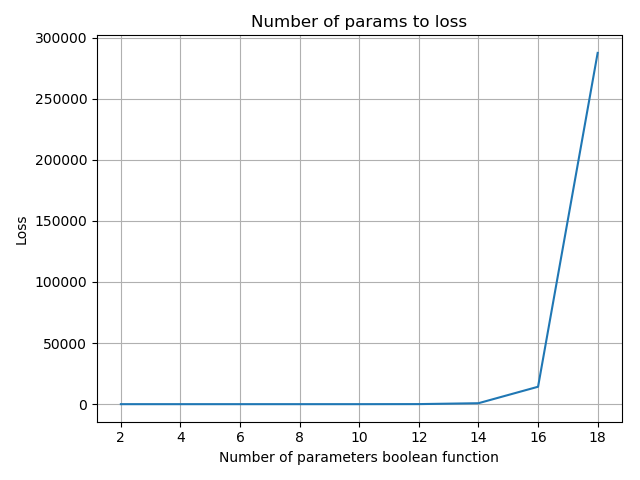
\includegraphics[width=\linewidth]{Loss_params.png}
	Рис. 2: График зависимости значений потерь от количества входных нейронов при $N_{in} = n$.
	
	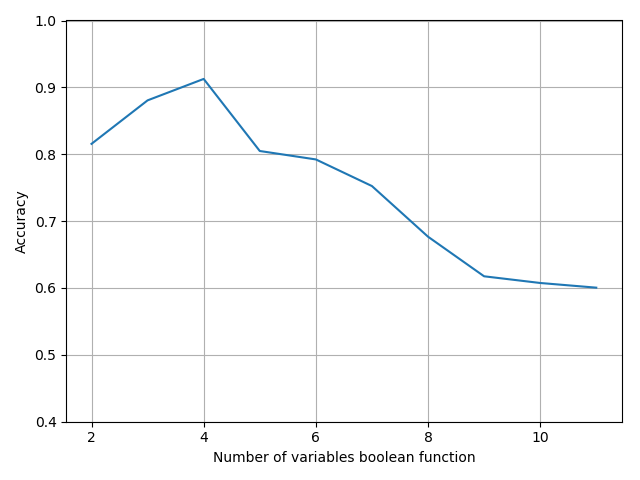
\includegraphics[width=\linewidth]{Accuracy_params_teta.png}
	Рис. 3: График зависимости точности построенной модели от количества входных нейронов при $N_{in} = \sum_{i=1}^k C_n^i$.
	
	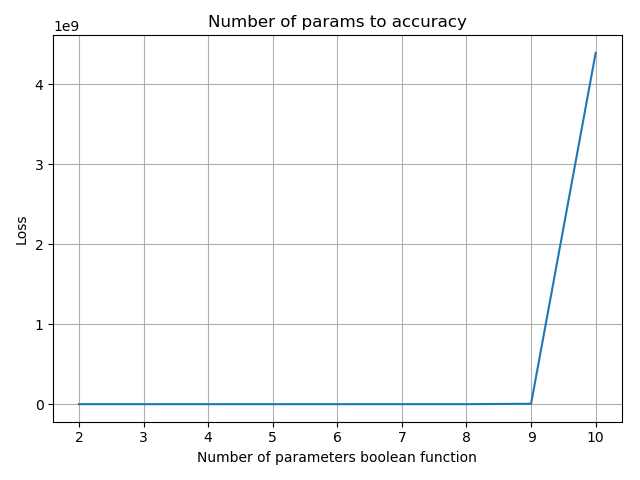
\includegraphics[width=\linewidth]{Loss_params_teta.png}
	Рис. 4: График зависимости значений потерь от количества входных нейронов при $N_{in} = \sum_{i=1}^k C_n^i$.

	Из полученных результатов, очевидно что следует использовать второй метод выбора количества нейронов на скрытых слоях. В дальнейшем будем использовать, данный метод.
	
	\subsection{Проведение компьютерных экспериментов на контрольных данных}
	Были проведены эксперимента для выборок $A_1$, $A_2$ и $A_3$.
	 
	
	\newpage	
	\section{Заключение}
	\bigskip
	В данной работе построены однослойная и многослойная нейронные сети для апроксимации бинарных функций. Для данных нейронных сетей были проведены компьютерные эксперименты и их последующий анализ. Были проведены различные эксперименты над нашей моделью, чтобы определить лучшую структуру и параметры.

	\newpage	
	\section*{Литература}
	\bigskip
	\begin{enumerate}
		\item Харин Ю.С., Берник В.И., Матвеев Г.В., Агиевич С.В. Математические и компьютерные основы криптологии. — 2003. — Минск.
		\item Neural networks in cryptography [Электрон. ресурс]. — 2015. — \\
		$\underline{http://cryptowiki.net/index.php?title=Neural\_networks\_in\_cryptography}$.
		\item Pattanayak S., Ludwig S.A. Encryption based on Neural Cryptography. — 2017.
		\item Kinzel F., Kanter I. Neural Cryptography. — 2002.
	\end{enumerate}
	

\end{document}
